\chapter{System Design}
Chapter introductory text here ...

\subsection{Pin Definition}
In the Figure \ref{fig-pin}, the pin definition of NodeMCU \cite{nodemcu2014} is shown and in  the Table \ref{table1} a detailed pin description is given. 
 
\begin{figure}[H]
\begin{center}
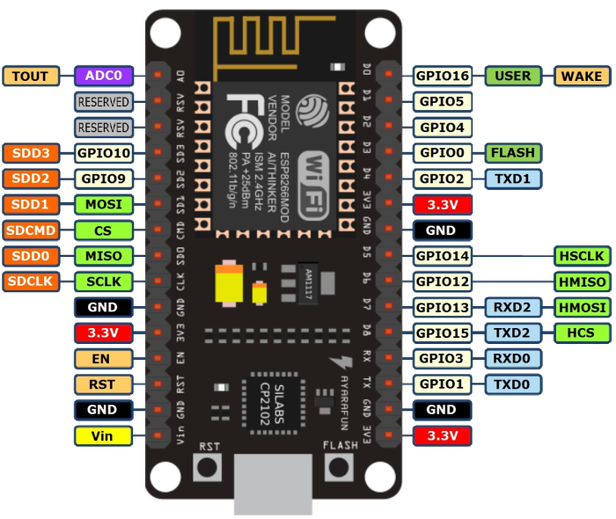
\includegraphics[width=0.66\textwidth]{figpin}
\end{center}
\caption{Pin Definition of NodeMCU}
\label{fig-pin}
\end{figure}

\begin{table}
\centering
\caption{Pin Description of NodeMCU}
\label{table1}
\begin{tabular}{|l|l|l|p{8cm}|}
\hline 
\textbf{Pin} & \textbf{Name} & \textbf{Type} & \textbf{Function} \tabularnewline
\hline 
1 & VDDA & P & Analog Power 3.02 \~ 3.6 V \tabularnewline \hline 
2 & LNA & I/O & RF Antenna Interface. Chip Output Impedance=50$\Omega$ No matching required but we recommend that the $\pi$-type matching network is retained. \tabularnewline \hline 
3 & VDD3P3 & P & Analog Power 3.02 \~ 3.6 V \tabularnewline \hline 
4 & VDD3P3 & P & Analog Power 3.02 \~ 3.6 V \tabularnewline \hline 
5 & VDD3P3 & P & Analog Power 3.02 \~ 3.6 V \tabularnewline \hline 
6 & ... & ... & ... \tabularnewline \hline 
\end{tabular}
\end{table}


\section{Parameter}
The NodeMCU parameters are listed in Table \ref{table2}.

\begin{table}
\caption{Parameters of NodeMCU}
\label{table2}
\centering
\begin{tabular}{|l|p{3.7cm}|p{4.8cm}|}
\hline 
\textbf{Categories} & \textbf{Items} & \textbf{Values} \tabularnewline
\hline 
\multirow{1}{*}{Wi-Fi Parameters} & certificates & FCC/CE/TELEC/SRRC \\\cline{2-3}
                 & WiFi Protocols & 802.11 b/g/n \\\cline{2-3}
                 & Frequency Range	 & 2.4G-2.5G (2400M-2483.5M) \\\cline{2-3}
                 & \multirow{2}{*}{TX Power} & 802.11 b: +20 dBm \\\cline{3-3}
                 & & 802.11 g: +17 dBm \\ \cline{3-3}
                 & & 802.11 n: +14 dBm \\ \cline{2-3}
                 & \multirow{2}{*}{RX Sensitivity} & 802.11 b: -91 dbm (11 Mbps)   \\\cline{3-3}
                 & & 802.11 g: -75 dbm (54 Mbps)  \\ \cline{3-3}
                 & & 802.11 n: -72 dbm (MCS7) \\ \cline{2-3}
                   & Types of Antenna & PCB Trace, External, IPEX Connector, Ceramic Chip    \\ \cline{1-3}
                 
\multirow{1}{*}{Hardware Parameters} & \multirow{2}{*}{TX Power} & UART/SDIO/SPI/I2C/ \newline I2S/IR Remote Control \\\cline{3-3}
                 &  & GPIO/PWM\\\cline{2-3}                
                 & Operating Voltage & 3.0~3.6V \\ \cline{2-3}
                 & Operating Current & Average value: 80mA \\ \cline{2-3}
                 & Operating Temperature Range& -40°~125° \\ \cline{2-3}
                 & Ambient Temperature Range & Normal temperature  \\\cline{2-3}
                 & Package Size & 5x5mm  \\ \cline{2-3}
                 & External Interface & N/A \\ \cline{1-3} \hline 
\end{tabular}
\end{table}

\section{Chapter Summary}
In this chapter, ...













